\chapter{Virtualización}

La virtualización es la utilización de un software para imitar las características de un hardware específico y utilizarlo para recrear un sistema real. Normalmente utilizamos la virtualización para crear “\textbf{máquinas virtuales}” simulando un equipo informático donde realizaremos la instalación de un sistema operativo.

El sistema de virtualización permite exprimir un único servidor hardware, ya que al crear distintas máquinas virtuales en él, nos va a permitir poder tener distintos sistemas, aplicaciones y servicios.

El software que ejecutamos en cada máquina virtual va a estar separada del hardware real, ya que se comunicará y usará el hardware virtual que se le ha asignado.

\section{Conceptos en virtualización}

A la hora de hacer uso de un sistema de virtualización existen dos conceptos básicos que debemos entender y no debemos de mezclar.

\begin{itemize}
    \item \textbf{Anfitrión}: Es el equipo donde se ejecuta el sistema de virtualización, que nos permitirá crear distintas máquinas virtualizadas.

    \item \textbf{Invitado/huésped}: En inglés el \textit{guest machine}, es la máquina virtual.

    \item \textbf{Hypervisor}: También conocido como “virtualizador”, es el software que crea y ejecuta las máquinas virtuales. Existen dos tipos de hypervisores:
    \begin{itemize}
        \item \textbf{Type-1} o \textbf{virtualización nativa}: El hypervisor corre directamente sobre el hardware físico del anfitrión y las máquinas virtuales se ejecutarán sobre el hypervisor. Este tipo de hypervisores son capaces de permitir que una máquina virtual interactúe directamente sobre el hardware real. Ejemplos: \href{https://en.wikipedia.org/wiki/Kernel-based_Virtual_Machine}{KVM}, \href{https://en.wikipedia.org/wiki/Proxmox_Virtual_Environment}{Proxmox}, \href{https://en.wikipedia.org/wiki/VMware_ESXi}{VMware ESXi}

        \item \textbf{Type-2}: Sobre el hardware físico se ejecuta un sistema operativo anfitrión, y sobre él se ejecuta una aplicación virtualizadora, como cualquier otro proceso. Las máquinas virtuales en este tipo no conocen nada del hardware real.
    \end{itemize}

    \item \textbf{Extensiones de virtualización}: Son extensiones de virtualización que tienen los procesadores y permiten la ejecución de un huésped sin penalización en la virtualización. La extensión de Intel se llama \textbf{Intel VT-x}, y en AMD se llama \textbf{AMD-V}. Existen otras extensiones especializadas que se llaman Intel VT-d y AMD-Vi.

    \begin{center}
        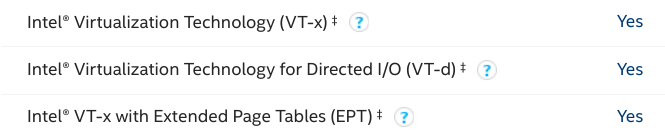
\includegraphics[frame,width=0.6\linewidth]{extension_intel.png}
    \end{center}
\end{itemize}

\section{Tipos de virtualización}
Cuando hablamos de virtualización podemos diferenciar distintos tipos, dependiendo de a qué nos refiramos, ya que existen virtualizaciones de todo tipo (plataformas hardware, recursos hardware, virtualización de almacenamiento, de red, ...).

Nos vamos a centrar en lo referente a virtualización de plataforma hardware, cuyo fin es el de crear máquinas virtuales. En este sentido podemos diferenciar dos tipos:

\begin{itemize}
    \item Virtualización completa
    \item Paravirtualización
\end{itemize}


El tipo más habitual es el de la virtualización completa, para el que hacemos uso de las \textbf{extensiones de virtualización} y que  conseguiremos que el rendimiento de la máquina sea mejor, ya que no va a haber prácticamente penalización.

Hoy día sólo podemos hacer uso de la paravirtualización con GNU/Linux.


